\documentclass[12pt]{article}
\usepackage{latexsym,amssymb,amsmath} % for \Box, \mathbb, split, etc.
% \usepackage[]{showkeys} % shows label names
\usepackage{cite} % sorts citation numbers appropriately
\usepackage{path}
\usepackage{url}
\usepackage{verbatim}
\usepackage[pdftex]{graphicx}

% horizontal margins: 1.0 + 6.5 + 1.0 = 8.5
\setlength{\oddsidemargin}{0.0in}
\setlength{\textwidth}{6.5in}
% vertical margins: 1.0 + 9.0 + 1.0 = 11.0
\setlength{\topmargin}{0.0in}
\setlength{\headheight}{12pt}
\setlength{\headsep}{13pt}
\setlength{\textheight}{625pt}
\setlength{\footskip}{24pt}

\renewcommand{\textfraction}{0.10}
\renewcommand{\topfraction}{0.85}
\renewcommand{\bottomfraction}{0.85}
\renewcommand{\floatpagefraction}{0.90}

\makeatletter
\setlength{\arraycolsep}{2\p@} % make spaces around "=" in eqnarray smaller
\makeatother

% change equation, table, figure numbers to be counted inside a section:
\numberwithin{equation}{section}
\numberwithin{table}{section}
\numberwithin{figure}{section}

% begin of personal macros
\newcommand{\half}{{\textstyle \frac{1}{2}}}
\newcommand{\eps}{\varepsilon}
\newcommand{\myth}{\vartheta}
\newcommand{\myphi}{\varphi}

\newcommand{\IN}{\mathbb{N}}
\newcommand{\IZ}{\mathbb{Z}}
\newcommand{\IQ}{\mathbb{Q}}
\newcommand{\IR}{\mathbb{R}}
\newcommand{\IC}{\mathbb{C}}
\newcommand{\Real}[1]{\mathrm{Re}\left({#1}\right)}
\newcommand{\Imag}[1]{\mathrm{Im}\left({#1}\right)}

\newcommand{\norm}[2]{\|{#1}\|_{{}_{#2}}}
\newcommand{\abs}[1]{\left|{#1}\right|}
\newcommand{\ip}[2]{\left\langle {#1}, {#2} \right\rangle}
\newcommand{\der}[2]{\frac{\partial {#1}}{\partial {#2}}}
\newcommand{\dder}[2]{\frac{\partial^2 {#1}}{\partial {#2}^2}}
\usepackage{enumitem}
\newcommand{\nn}{\mathbf{n}}
\newcommand{\xx}{\mathbf{x}}
\newcommand{\uu}{\mathbf{u}}
\usepackage{tikz}
\usetikzlibrary{arrows}
\usetikzlibrary{positioning}
\usepackage{titlesec}
\newcommand{\junk}[1]{{}}
\usepackage{xcolor}
\definecolor{darkblue}{rgb}{0,0,0.4}
\usepackage[colorlinks = true,
linkcolor = darkblue,
urlcolor  = darkblue,
citecolor = darkblue,
anchorcolor = darkblue]{hyperref}
% set two lengths for the includegraphics commands used to import the plots:
\newlength{\fwtwo} \setlength{\fwtwo}{0.45\textwidth}
% end of personal macros

\begin{document}
\DeclareGraphicsExtensions{.jpg}

\begin{center}
\textsc{\Large Statistical Pattern Recognition} \\[2pt]
	\textsc{\large Assignment 1}\\
	\vspace{0.5cm}
  Ali Gholami \\[6pt]
  Department of Computer Engineering \& Information Technology\\
  Amirkabir University of Technology  \\[6pt]
  \def\UrlFont{\em}
  \url{http://ceit.aut.ac.ir/~aligholamee}\\
    \href{mailto:aligholamee@aut.ac.ir}{\textit{aligholamee@aut.ac.ir}}
\end{center}

\begin{abstract}
This is an introductory assignment to the world of \textit{Statistics} and \textit{Probability} in the world of \textit{Pattern Recognition}. We'll introduce some key concepts like \textit{Probability Distribution Function, Cumulative Distribution Function, Probability Density Function, Probability Mass Function, Joint Probability Density Function, Joint Cumulative Density Function, Marginal Density} \& more details as the probabilistic point of view. Furthermore, we'll review the concepts of \textit{Expected Value, Variance, Standard Deviation, Covariance \& Correlation of Random Variables(e.g. Random Vectors), Univariate \& Multivariate Gaussian Distribution, Total Probability \& Bayes Theorem, Geometric \& Mahalanobis Distances, Central Limit Theorem, Independence \& Correlation} as the statistics point of view. Also, a principal concept called \textit{Linear Transformation} is discussed. The relationship between these fields is far more important than each separately.
\end{abstract}

\subparagraph{Key Words.} \textit{PDF, PMF, JPDF, JPMF, CDF, JCDF, Covariance Matrix, Correlation Coefficient, Correlation, Variance, Expected Vector, Gaussian Distribution, Marginal Probability, Linear Tranformation, Eigenvector, Eigenvalue, Rank.}

\subsection{1. Expectation Properties}

A random variable \textit{$X$} has \textit{$E(X) = -4$} and \textit{E($X^2$) = 30.} Let \textit{$Y = -3X + 7$.} Compute the following.

\begin{enumerate}[label=(\alph*)]
	\item \textit{$V(X)$}
	
	\item \textit{$V(Y)$}
	
	\item \textit{$E((X+5)^2)$}
	
	\item \textit{$E(Y^2)$}
	
\end{enumerate}


\begin{figure} \centering
	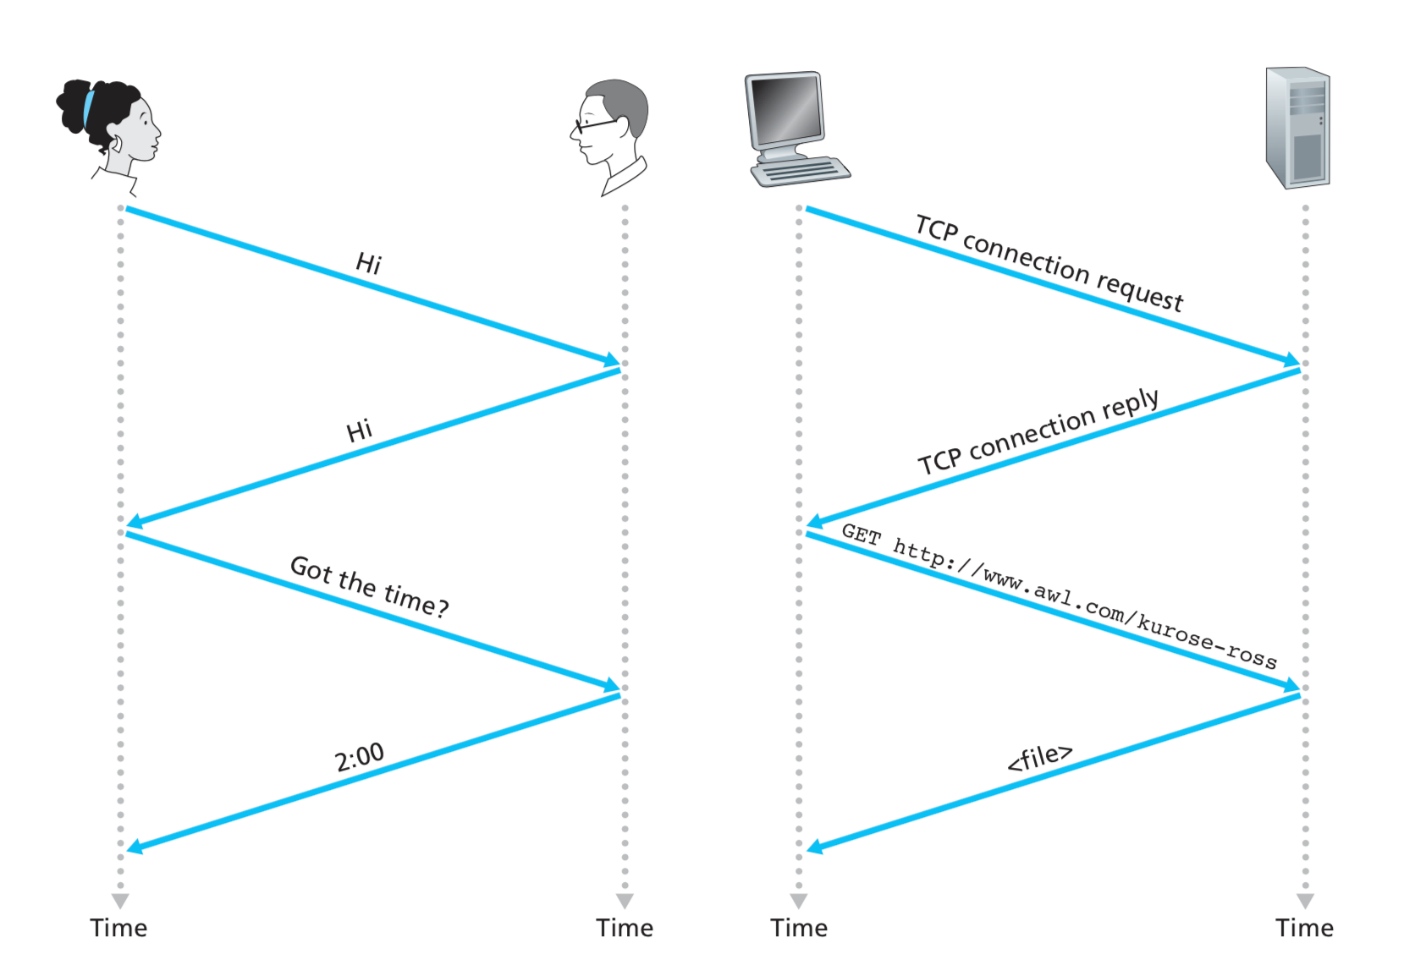
\includegraphics[width=0.7\textwidth]{figconvrateloglog}
	\caption{TCP connection request sample}
	\label{figsolplot}
\end{figure}
\titleformat{\section}
{\normalfont\Large\bfseries}   % The style of the section title
{}                             % a prefix
{0pt}                          % How much space exists between the prefix and the title
{Section \thesection:\quad}    % How the section is represented
\subsection{Solution}

Assuming the data is transferred via \textit{packets}, a label has to be given to each packet of data. These labels are called \textit{headers}. The objective of these headers is to provide some information about each of these packets of data. These information include \textit{source and destination nodes address, class of message(including the objective codes, message origin, class functions).} In addition to that, the main \textit{data elements} are present in each packet. We'll propose a high-level abstraction of protocol classes below. Each of these classes specifies the overall purpose of the message.\\
\\

\begin{enumerate}
	\item{Authorization Message}
		\begin{itemize}
			\item{Authorize the card pass phrase}
			\item{Determine if funds are available}
			\item{Determine if the destination card exists in a card-to-card transaction}
		\end{itemize}
		
	\item{Financial Message}
		\begin{itemize}
			\item{Post funds to the accounts in card-to-card transactions}
			\item{Post funds to the accounts in \textit{POS} transactions}
			\item{Fund posting approvals}
		\end{itemize}
	
	\item{Reversal \& Rollback Message}
		\begin{itemize}
			\item{Reverse the previous authorization action}
			\item{Rollback the previous financial message}
		\end{itemize}
		
	\item{Administrative Message}
		\begin{itemize}
			\item{Transmit the administrative messages and advices}
			\item{Public announcements on the \textit{ATM}}
		\end{itemize}
		
	\item{Network Management Message}
		\begin{itemize}
			\item{Secure key exchange}
		\end{itemize}
	
\end{enumerate}

\begin{table} \centering
	\begin{tabular}{rcccc}
		\hline
		$ Message $ &
		$ Action$ & $ Device $ \\
		\hline
		 Authorization & Request for authorization & ATM \\
		 Authorization & Repeat authorization request & ATM\\
		 Authorization & Respond to authorization request & Central Computer\\
		 Financial & Request for fund & ATM \\
		 Financial & Repeat fund request & ATM \\
		 Financial & Respond to financial request & Central Computer \\
		 Financial & Request for account report & ATM \\
		 Financial & Respond to account report & Central Computer \\
		 Reversal & Reverse a card-to-card transaction & ATM \\
		 Reversal & Rollback a card-to-card transaction & ATM \\
		 Administrative & Request for public announcement due date & ATM \\
		 Administrative & Respond to the public announcement & Central Computer \\
		 Network Management & Echo test & ATM \\
		 Network Management & Respond to Echo test & Central Computer\\
		 
		 
		\hline
	\end{tabular}
	\caption{Demonstration of proposed \textit{ATM} network protocol classes.}
	\label{tabconvdemo}
\end{table}

A complete example of a fund request is described in the figure 1.2. \textbf{Firstly}, the \textit{ATM} sends an authorization request to the central computer. \textbf{Secondly}, The central computer responds to the incoming request. \textbf{Thirdly}, in case the authorization is successful, a fund request is sent to the central computer. \textbf{Fourthly}, the fund request is validated and the reponse is sent to the \textit{ATM}. In the situation, the user might ask for a reversal. If that happens, the reversal requests/responses are transferred.

\begin{figure}[!h]
	\centering
		\begin{tikzpicture}[scale=1]
		\tikzstyle{ann} = [draw=none,fill=none,right]
		\matrix[nodes={draw, ultra thick, fill=blue!10},
		row sep=1.5cm,column sep=2cm] {
			\node[rectangle] (a1) {ATM - Request for authentication}; &
			\node[rectangle] (c1) {Computer - Authentication reponse};\\
			\node[rectangle] (a2) {ATM - Request for fund}; &
			\node[rectangle] (c2) {Computer - Fund reponse};\\
			\node[rectangle] (a3) {ATM - Request for account report}; &
			\node[rectangle] (c3) {Computer - Account report reponse};\\
		};
		
			\draw [->] [line width=2pt, -stealth](a1) to [bend left=15] node{} (c1);
			\draw [->] [line width=2pt, -stealth](c1) to [bend left=15] node{} (a1);
			
			\draw [->] [line width=2pt, -stealth](a2) to [bend left=15] node{} (c2);
			\draw [->] [line width=2pt, -stealth](c2) to [bend left=15] node{} (a2);

			\draw [->] [line width=2pt, -stealth](a3) to [bend left=15] node{} (c3);
			\draw [->] [line width=2pt, -stealth](c3) to [bend left=15] node{} (a3);

		\end{tikzpicture}
		
		\caption{A complete fund request flow diagram.}
		\label{tabconvdemo}
\end{figure}

Please refer to the beginning of this solution for the assumptions about the \textit{transport} layer.

\titleformat{\section}
{\normalfont\Large\bfseries}   % The style of the section title
{}                             % a prefix
{0pt}                          % How much space exists between the prefix and the title
{Section \thesection:\quad}    % How the section is represented

\subsection{2. HFC \& Collision in Downstream}
Given an \textit{HFC} communication medium, find out whether the transmission rate is \textit{dedicated} to one user or it is shared among users in the network. Is it possible for a downstream in an \textit{HFC} channel to have collision? Describe your answer.

\subsection{Solution}

As the description for the \textit{HFC(Hybrid fiber-coaxial)} medium specifies, the combination of both \textit{optical fiber} and \textit{coaxial cable} is used in a broadband network. As an example for the functionality of this medium, the television channels are sent from the cable system's distribution facility, the \textit{\textbf{headend}}, to local communities through optical fiber subscriber lines. At the local community, a box called an \textit{optical node} translates the signal from a light beam to electrical signal, and sends it over coaxial cable lines for distribution to subscriber residences.\\
\subparagraph{HFC Transmission Rate }HFC bandwidth is shared among users. So, each user on a tail-end of the coaxial cable can use the same transmission rate as others.\\
\subparagraph{Collision in Downstream}

The downstream channel, provides the data from a single source called head-end. Then the data is distributed among the residences. Thus, there are no collisions in the downstream channel.
\\


\subsection{3. Dial-up, ADSL, FTTH, HFC Modems}
The modems titled here are widely used as a home-access to the Internet. Provide an example of \textit{maximum transmission rate}. Describe whether these rates are shared or not.

\subsection{Solution}

Table 1.2 provides various \textit{transmission rates(Bitrate)} for each of these modems.

\begin{table}[!h]
	\centering
	\begin{tabular}{rcccc}
		\hline
		$ Modem $ &
		$ Bitrate $ & $ Usage $ \\
		\hline
		Dial-up & 33.6(kbit/s) -- 48(kbit/s) -- 56(kbit/s) & Unshared \\
		ADSL & 8.0(Mbit/s) -- 12.0(Mbit/s) -- 24(Mbit/s) & Unshared -- Shared\\
		HFC &  100(Mbit/s) & Shared\\
		FTTH & 1(Gbit/s)(Google Fiber) & Unshared(one single home)\\
		\hline
	\end{tabular}
	\caption{Bitrate samples for different types of modems.}
	\label{tabconvdemo}
\end{table}

\end{document}